\documentclass[12pt]{article}

\usepackage[spanish]{babel}
\usepackage{hyperref}
\usepackage{graphicx}
\usepackage{listings}
\usepackage{color}
\usepackage{multicol}
\usepackage{amssymb}
\usepackage{enumitem}
\usepackage{here}
\usepackage{dsfont}
\usepackage{amsmath}
\usepackage{tipa}
\usepackage{float}
\spanishdecimal{.}

\title{Matemáticas para las Ciencias Aplicadas I}
\title{
	Tercera Lista de Problemas \\
	\textbf{Segunda  Parte} \\
	\vspace{1ex}
	\large Matemáticas para las Ciencias Aplicadas I \\
	Facultad de Ciencias, UNAM}

\date{\today}

\author{Flores Morán Julieta Melina \\ Zarco Romero José Antonio}

\begin{document}

\maketitle

%% De la sección 4.1: ejercicios 31, 57 y 71.
%% De la sección 4.2: ejercicios 31, 55 y 77.
%% De la sección 4.3: ejercicios 21, 36, 54 y 70.

%% 4.1 -----------------------------------------------------------------------------------------------------------------------------------------------------------------------------------------------------------------------------
\section{Sección 4.1 \\ Análisis De Funciones I: Aumento, Disminución Y Concavidad}
% 31 -------------------------------------------------------------------------------------------------------------
\subsection{Ejercicio 31} name \\

Encuentre: (a) los intervalos en los que $f$ aumenta, (b) los intervalos en los que $f$ disminuye, (c) los intervalos abiertos en los que $f$ es cóncava hacia arriba, (d) los intervalos abiertos en los que $f$ es cóncava hacia abajo, y (e) las coordenadas x de todos los puntos de inflexión.
\[
f(x) = \tan^{-1}(x^2-1)
\]

% 57 -------------------------------------------------------------------------------------------------------------
\subsection{Ejercicio 57} name \\

\begin{enumerate}[label=(\alph*)]
\item Demuestre que un polinomio cúbico general
  \[
  f(x) = ax^3 + bx^2 + cx + d \qquad (a\neq 0)
  \]
  tiene exactamente un punto de inflexión.

\item Demuestre que si un polinomio cúbico tiene tres intersecciones en el eje x, entonces el punto de inflexión ocurre en el valor promedio de las intersecciones.

\item Utilice el resultado del inciso (b) para encontrar el punto de inflexión del polinomio cúbico $f(x) = x^3-3x^2 + 2x$, y verifique su resultado usando $f''$ para determinar dónde $f$ es cóncava hacia arriba y cóncava hacia abajo.
  
\end{enumerate}

% 71 -------------------------------------------------------------------------------------------------------------
\subsection{Ejercicio 71} name \\

Suponiendo que $A, k$ y $L$ son constantes positivas, verifique que la gráfica de $y=L/(1+Ae^{-kt})$ tiene un punto de inflexión en $\left( \frac{1}{k}\ln{A},\frac{1}{2}L \right)$.


%% 4.2 -----------------------------------------------------------------------------------------------------------------------------------------------------------------------------------------------------------------------------
\section{Sección 4.2 \\ Análisis De Funciones II: Extremos Relativos; Graficar Polinomios} 
% 31 -------------------------------------------------------------------------------------------------------------
\subsection{Ejercicio 31} name \\

Utilice la derivada dada para encontrar todos los puntos críticos de $f$ y en cada punto crítico determine si ocurre un máximo relativo, un mínimo relativo o ninguno de los dos. Supongamos en cada caso que $f$ es continua en todas partes.
\[
f'(x)=\ln{\left( \frac{2}{1+x^2} \right)}
\]

% 55 -------------------------------------------------------------------------------------------------------------
\subsection{Ejercicio 55} name \\

Haz una gráfica del polinomio y etiqueta las coordenadas de las intersecciones, los puntos estacionarios y los puntos de inflexión. Comprueba tu trabajo con una utilidad gráfica.
\[
p(x) = (x + 1)^2 (2x-x^2 )
\]

% 77 -------------------------------------------------------------------------------------------------------------
\subsection{Ejercicio 77} name \\

En cada parte, encuentre $k$ de modo que $f$ tenga un extremo relativo en el punto donde $x = 3$.
\begin{enumerate}[label=(\alph*)]
\item $f(x)=x^2+\frac{k}{x}$
\item $f(x)=\frac{x}{x^2+k}$
\end{enumerate}

%% 4.3 -----------------------------------------------------------------------------------------------------------------------------------------------------------------------------------------------------------------------------
\section{Sección 4.3 \\  Análisis De Funciones III: Funciones Racionales, Cúspides Y Tangentes Verticales}
% 21 -------------------------------------------------------------------------------------------------------------
\subsection{Ejercicio 21} name \\

Dibuja una gráfica de la función racional y etiqueta las coordenadas de los puntos estacionarios y los puntos de inflexión. Muestra las asíntotas horizontales, verticales, oblicuas y curvilíneas y etiquétalas con sus ecuaciones. Etiquete los puntos, si los hay, donde la gráfica cruza una asíntota. Comprueba tu trabajo con una utilidad gráfica.
\[
\frac{(x-2)^3}{x^2}
\]

% 36 -------------------------------------------------------------------------------------------------------------
\subsection{Ejercicio 36} name \\

Dé una gráfica de la función e identifique las ubicaciones de todos los puntos críticos y puntos de inflexión. Comprueba tu trabajo con una utilidad gráfica.
\[
5x^{2/3}+x^{5/3}
\]

% 54 -------------------------------------------------------------------------------------------------------------
\subsection{Ejercicio 54} name \\

Utilizando la regla de L'Hôpital se puede verificar que
\begin{align*}
  \lim_{x \to +\infty} \frac{e^x}{x}=+\infty && \lim_{x \to +\infty} \frac{x}{e^x}=0 && \lim_{x \to -\infty} xe^x=0
\end{align*}
En estos ejercicios: (a) Utilice estos resultados, según sea necesario, para encontrar los límites de $f(x)$ cuando $x\rightarrow +\infty$ y cuando $x\rightarrow -\infty$. (b) Dibuje una gráfica de $f(x)$ e identifique todos los extremos relativos, puntos de inflexión y asíntotas (según corresponda). Comprueba tu trabajo con una utilidad gráfica.
\[
f(x)=x^3e^{x-1}
\]

% 70 -------------------------------------------------------------------------------------------------------------
\subsection{Ejercicio 70} name \\

La figura adjunta muestra una gráfica generada por computadora del polinomio $y = 0.1x^5 (x + 1)^2$ usando una ventana de visualización de $[−2, 1.5] \times [−0.2, 0.2]$. Demuestre que la elección de la escala vertical hizo que la computadora pasara por alto características importantes de la gráfica. Encuentra las características que faltaron y haz tu propio boceto del gráfico que muestra las características que faltan.
\begin{figure}[H]
\centering
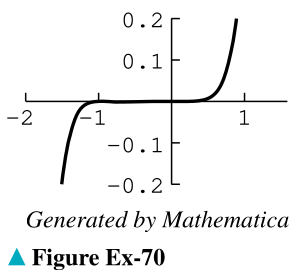
\includegraphics[width=0.4\textwidth]{../img/img_Lista3/2_70.png}
\end{figure}

\end{document}
